% Options for packages loaded elsewhere
% Options for packages loaded elsewhere
\PassOptionsToPackage{unicode}{hyperref}
\PassOptionsToPackage{hyphens}{url}
\PassOptionsToPackage{dvipsnames,svgnames,x11names}{xcolor}
%
\documentclass[
  letterpaper,
  DIV=11,
  numbers=noendperiod]{scrartcl}
\usepackage{xcolor}
\usepackage{amsmath,amssymb}
\setcounter{secnumdepth}{-\maxdimen} % remove section numbering
\usepackage{iftex}
\ifPDFTeX
  \usepackage[T1]{fontenc}
  \usepackage[utf8]{inputenc}
  \usepackage{textcomp} % provide euro and other symbols
\else % if luatex or xetex
  \usepackage{unicode-math} % this also loads fontspec
  \defaultfontfeatures{Scale=MatchLowercase}
  \defaultfontfeatures[\rmfamily]{Ligatures=TeX,Scale=1}
\fi
\usepackage{lmodern}
\ifPDFTeX\else
  % xetex/luatex font selection
\fi
% Use upquote if available, for straight quotes in verbatim environments
\IfFileExists{upquote.sty}{\usepackage{upquote}}{}
\IfFileExists{microtype.sty}{% use microtype if available
  \usepackage[]{microtype}
  \UseMicrotypeSet[protrusion]{basicmath} % disable protrusion for tt fonts
}{}
\makeatletter
\@ifundefined{KOMAClassName}{% if non-KOMA class
  \IfFileExists{parskip.sty}{%
    \usepackage{parskip}
  }{% else
    \setlength{\parindent}{0pt}
    \setlength{\parskip}{6pt plus 2pt minus 1pt}}
}{% if KOMA class
  \KOMAoptions{parskip=half}}
\makeatother
% Make \paragraph and \subparagraph free-standing
\makeatletter
\ifx\paragraph\undefined\else
  \let\oldparagraph\paragraph
  \renewcommand{\paragraph}{
    \@ifstar
      \xxxParagraphStar
      \xxxParagraphNoStar
  }
  \newcommand{\xxxParagraphStar}[1]{\oldparagraph*{#1}\mbox{}}
  \newcommand{\xxxParagraphNoStar}[1]{\oldparagraph{#1}\mbox{}}
\fi
\ifx\subparagraph\undefined\else
  \let\oldsubparagraph\subparagraph
  \renewcommand{\subparagraph}{
    \@ifstar
      \xxxSubParagraphStar
      \xxxSubParagraphNoStar
  }
  \newcommand{\xxxSubParagraphStar}[1]{\oldsubparagraph*{#1}\mbox{}}
  \newcommand{\xxxSubParagraphNoStar}[1]{\oldsubparagraph{#1}\mbox{}}
\fi
\makeatother

\usepackage{color}
\usepackage{fancyvrb}
\newcommand{\VerbBar}{|}
\newcommand{\VERB}{\Verb[commandchars=\\\{\}]}
\DefineVerbatimEnvironment{Highlighting}{Verbatim}{commandchars=\\\{\}}
% Add ',fontsize=\small' for more characters per line
\usepackage{framed}
\definecolor{shadecolor}{RGB}{241,243,245}
\newenvironment{Shaded}{\begin{snugshade}}{\end{snugshade}}
\newcommand{\AlertTok}[1]{\textcolor[rgb]{0.68,0.00,0.00}{#1}}
\newcommand{\AnnotationTok}[1]{\textcolor[rgb]{0.37,0.37,0.37}{#1}}
\newcommand{\AttributeTok}[1]{\textcolor[rgb]{0.40,0.45,0.13}{#1}}
\newcommand{\BaseNTok}[1]{\textcolor[rgb]{0.68,0.00,0.00}{#1}}
\newcommand{\BuiltInTok}[1]{\textcolor[rgb]{0.00,0.23,0.31}{#1}}
\newcommand{\CharTok}[1]{\textcolor[rgb]{0.13,0.47,0.30}{#1}}
\newcommand{\CommentTok}[1]{\textcolor[rgb]{0.37,0.37,0.37}{#1}}
\newcommand{\CommentVarTok}[1]{\textcolor[rgb]{0.37,0.37,0.37}{\textit{#1}}}
\newcommand{\ConstantTok}[1]{\textcolor[rgb]{0.56,0.35,0.01}{#1}}
\newcommand{\ControlFlowTok}[1]{\textcolor[rgb]{0.00,0.23,0.31}{\textbf{#1}}}
\newcommand{\DataTypeTok}[1]{\textcolor[rgb]{0.68,0.00,0.00}{#1}}
\newcommand{\DecValTok}[1]{\textcolor[rgb]{0.68,0.00,0.00}{#1}}
\newcommand{\DocumentationTok}[1]{\textcolor[rgb]{0.37,0.37,0.37}{\textit{#1}}}
\newcommand{\ErrorTok}[1]{\textcolor[rgb]{0.68,0.00,0.00}{#1}}
\newcommand{\ExtensionTok}[1]{\textcolor[rgb]{0.00,0.23,0.31}{#1}}
\newcommand{\FloatTok}[1]{\textcolor[rgb]{0.68,0.00,0.00}{#1}}
\newcommand{\FunctionTok}[1]{\textcolor[rgb]{0.28,0.35,0.67}{#1}}
\newcommand{\ImportTok}[1]{\textcolor[rgb]{0.00,0.46,0.62}{#1}}
\newcommand{\InformationTok}[1]{\textcolor[rgb]{0.37,0.37,0.37}{#1}}
\newcommand{\KeywordTok}[1]{\textcolor[rgb]{0.00,0.23,0.31}{\textbf{#1}}}
\newcommand{\NormalTok}[1]{\textcolor[rgb]{0.00,0.23,0.31}{#1}}
\newcommand{\OperatorTok}[1]{\textcolor[rgb]{0.37,0.37,0.37}{#1}}
\newcommand{\OtherTok}[1]{\textcolor[rgb]{0.00,0.23,0.31}{#1}}
\newcommand{\PreprocessorTok}[1]{\textcolor[rgb]{0.68,0.00,0.00}{#1}}
\newcommand{\RegionMarkerTok}[1]{\textcolor[rgb]{0.00,0.23,0.31}{#1}}
\newcommand{\SpecialCharTok}[1]{\textcolor[rgb]{0.37,0.37,0.37}{#1}}
\newcommand{\SpecialStringTok}[1]{\textcolor[rgb]{0.13,0.47,0.30}{#1}}
\newcommand{\StringTok}[1]{\textcolor[rgb]{0.13,0.47,0.30}{#1}}
\newcommand{\VariableTok}[1]{\textcolor[rgb]{0.07,0.07,0.07}{#1}}
\newcommand{\VerbatimStringTok}[1]{\textcolor[rgb]{0.13,0.47,0.30}{#1}}
\newcommand{\WarningTok}[1]{\textcolor[rgb]{0.37,0.37,0.37}{\textit{#1}}}

\usepackage{longtable,booktabs,array}
\usepackage{calc} % for calculating minipage widths
% Correct order of tables after \paragraph or \subparagraph
\usepackage{etoolbox}
\makeatletter
\patchcmd\longtable{\par}{\if@noskipsec\mbox{}\fi\par}{}{}
\makeatother
% Allow footnotes in longtable head/foot
\IfFileExists{footnotehyper.sty}{\usepackage{footnotehyper}}{\usepackage{footnote}}
\makesavenoteenv{longtable}
\usepackage{graphicx}
\makeatletter
\newsavebox\pandoc@box
\newcommand*\pandocbounded[1]{% scales image to fit in text height/width
  \sbox\pandoc@box{#1}%
  \Gscale@div\@tempa{\textheight}{\dimexpr\ht\pandoc@box+\dp\pandoc@box\relax}%
  \Gscale@div\@tempb{\linewidth}{\wd\pandoc@box}%
  \ifdim\@tempb\p@<\@tempa\p@\let\@tempa\@tempb\fi% select the smaller of both
  \ifdim\@tempa\p@<\p@\scalebox{\@tempa}{\usebox\pandoc@box}%
  \else\usebox{\pandoc@box}%
  \fi%
}
% Set default figure placement to htbp
\def\fps@figure{htbp}
\makeatother





\setlength{\emergencystretch}{3em} % prevent overfull lines

\providecommand{\tightlist}{%
  \setlength{\itemsep}{0pt}\setlength{\parskip}{0pt}}



 


\KOMAoption{captions}{tableheading}
\makeatletter
\@ifpackageloaded{caption}{}{\usepackage{caption}}
\AtBeginDocument{%
\ifdefined\contentsname
  \renewcommand*\contentsname{Table of contents}
\else
  \newcommand\contentsname{Table of contents}
\fi
\ifdefined\listfigurename
  \renewcommand*\listfigurename{List of Figures}
\else
  \newcommand\listfigurename{List of Figures}
\fi
\ifdefined\listtablename
  \renewcommand*\listtablename{List of Tables}
\else
  \newcommand\listtablename{List of Tables}
\fi
\ifdefined\figurename
  \renewcommand*\figurename{Figure}
\else
  \newcommand\figurename{Figure}
\fi
\ifdefined\tablename
  \renewcommand*\tablename{Table}
\else
  \newcommand\tablename{Table}
\fi
}
\@ifpackageloaded{float}{}{\usepackage{float}}
\floatstyle{ruled}
\@ifundefined{c@chapter}{\newfloat{codelisting}{h}{lop}}{\newfloat{codelisting}{h}{lop}[chapter]}
\floatname{codelisting}{Listing}
\newcommand*\listoflistings{\listof{codelisting}{List of Listings}}
\makeatother
\makeatletter
\makeatother
\makeatletter
\@ifpackageloaded{caption}{}{\usepackage{caption}}
\@ifpackageloaded{subcaption}{}{\usepackage{subcaption}}
\makeatother
\usepackage{bookmark}
\IfFileExists{xurl.sty}{\usepackage{xurl}}{} % add URL line breaks if available
\urlstyle{same}
\hypersetup{
  pdftitle={Phloem metabolites and seed composition},
  pdfauthor={Juan Ignacio Zucchetti},
  colorlinks=true,
  linkcolor={blue},
  filecolor={Maroon},
  citecolor={Blue},
  urlcolor={Blue},
  pdfcreator={LaTeX via pandoc}}


\title{Phloem metabolites and seed composition}
\author{Juan Ignacio Zucchetti}
\date{}
\begin{document}
\maketitle


\subsection{Biological background}\label{biological-background}

Phloem-delivered metabolites were measured in six contrasting soybean
genotypes at two developmental stages (R5 and R6). Pearson correlations
were calculated between phloem metabolite levels and final seed
composition (protein content, protein concentration, oil concentration,
seed weight).

\subsection{Results}\label{results}

\subsubsection{Early seed filling (R5)}\label{early-seed-filling-r5}

\begin{Shaded}
\begin{Highlighting}[]
\FunctionTok{library}\NormalTok{(tinytex)}
\end{Highlighting}
\end{Shaded}

\begin{verbatim}
Warning: package 'tinytex' was built under R version 4.5.3
\end{verbatim}

\begin{Shaded}
\begin{Highlighting}[]
\CommentTok{\#| echo: false}
\CommentTok{\#| message: false}
\CommentTok{\#| warning: false}
\FunctionTok{library}\NormalTok{(tidyverse)}
\end{Highlighting}
\end{Shaded}

\begin{verbatim}
Warning: package 'tidyverse' was built under R version 4.5.3
\end{verbatim}

\begin{verbatim}
Warning: package 'tidyr' was built under R version 4.5.2
\end{verbatim}

\begin{verbatim}
Warning: package 'readr' was built under R version 4.5.2
\end{verbatim}

\begin{verbatim}
Warning: package 'purrr' was built under R version 4.5.2
\end{verbatim}

\begin{verbatim}
Warning: package 'stringr' was built under R version 4.5.2
\end{verbatim}

\begin{verbatim}
Warning: package 'forcats' was built under R version 4.5.2
\end{verbatim}

\begin{verbatim}
Warning: package 'lubridate' was built under R version 4.5.2
\end{verbatim}

\begin{verbatim}
-- Attaching core tidyverse packages ------------------------ tidyverse 2.0.0 --
v dplyr     1.1.4     v readr     2.1.6
v forcats   1.0.1     v stringr   1.6.0
v ggplot2   3.5.2     v tibble    3.3.0
v lubridate 1.9.4     v tidyr     1.3.2
v purrr     1.2.1     
-- Conflicts ------------------------------------------ tidyverse_conflicts() --
x dplyr::filter() masks stats::filter()
x dplyr::lag()    masks stats::lag()
i Use the conflicted package (<http://conflicted.r-lib.org/>) to force all conflicts to become errors
\end{verbatim}

\begin{Shaded}
\begin{Highlighting}[]
\NormalTok{top\_R5 }\OtherTok{\textless{}{-}} \FunctionTok{read.csv}\NormalTok{(}\StringTok{"outputs/tables/top\_correlations\_R5.csv"}\NormalTok{)}
\NormalTok{knitr}\SpecialCharTok{::}\FunctionTok{kable}\NormalTok{(top\_R5)}
\end{Highlighting}
\end{Shaded}

\begin{longtable}[]{@{}llrrr@{}}
\toprule\noalign{}
metabolite & composition\_var & r & p & abs\_r \\
\midrule\noalign{}
\endhead
\bottomrule\noalign{}
\endlastfoot
met\_11 & Oil\_concentration & -0.5099202 & 0.0306278 & 0.5099202 \\
met\_17 & Oil\_concentration & -0.4934421 & 0.0374355 & 0.4934421 \\
met\_11 & Protein\_concentration & 0.7042599 & 0.0011039 & 0.7042599 \\
met\_09 & Protein\_concentration & 0.6006076 & 0.0083959 & 0.6006076 \\
met\_15 & Protein\_concentration & 0.5998491 & 0.0085004 & 0.5998491 \\
met\_32 & Protein\_concentration & 0.5904943 & 0.0098776 & 0.5904943 \\
met\_25 & Protein\_concentration & 0.5766655 & 0.0122358 & 0.5766655 \\
met\_09 & Protein\_content & 0.7619911 & 0.0002376 & 0.7619911 \\
met\_01 & Protein\_content & 0.6014610 & 0.0082795 & 0.6014610 \\
met\_15 & Protein\_content & 0.5496969 & 0.0181172 & 0.5496969 \\
met\_05 & Protein\_content & 0.5343685 & 0.0223395 & 0.5343685 \\
met\_25 & Protein\_content & 0.5160816 & 0.0283447 & 0.5160816 \\
met\_09 & Seed\_weight & 0.6523641 & 0.0033427 & 0.6523641 \\
met\_33 & Seed\_weight & 0.5425861 & 0.0199896 & 0.5425861 \\
met\_01 & Seed\_weight & 0.5392788 & 0.0209108 & 0.5392788 \\
met\_05 & Seed\_weight & 0.4945696 & 0.0369356 & 0.4945696 \\
\end{longtable}

\begin{center}
\pandocbounded{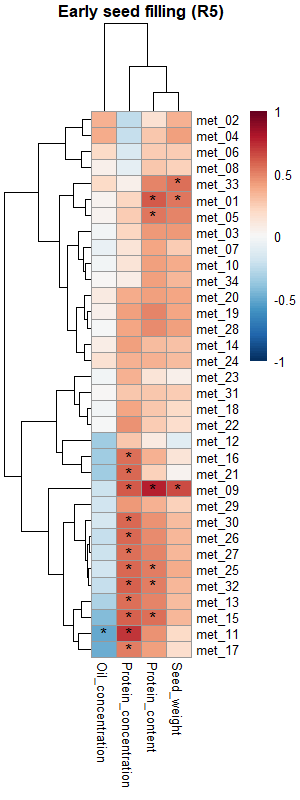
\includegraphics[keepaspectratio]{outputs/figures/heatmap_R5.png}}
\end{center}

\_\_\_\_\_\_\_\_\_\_\_\_\_\_\_\_

\subsubsection{Mid-Stage seed filling
(R6)}\label{mid-stage-seed-filling-r6}

\begin{longtable}[]{@{}llrrr@{}}
\toprule\noalign{}
metabolite & composition\_var & r & p & abs\_r \\
\midrule\noalign{}
\endhead
\bottomrule\noalign{}
\endlastfoot
met\_30 & Oil\_concentration & -0.4825902 & 0.0425157 & 0.4825902 \\
met\_15 & Protein\_concentration & 0.6738183 & 0.0021692 & 0.6738183 \\
met\_21 & Protein\_concentration & 0.6144973 & 0.0066581 & 0.6144973 \\
met\_26 & Protein\_concentration & 0.6080936 & 0.0074189 & 0.6080936 \\
met\_27 & Protein\_concentration & 0.6054476 & 0.0077531 & 0.6054476 \\
met\_12 & Protein\_concentration & 0.5975694 & 0.0088208 & 0.5975694 \\
met\_17 & Protein\_content & 0.7274079 & 0.0006239 & 0.7274079 \\
met\_27 & Protein\_content & 0.7023939 & 0.0011532 & 0.7023939 \\
met\_32 & Protein\_content & 0.6752665 & 0.0021043 & 0.6752665 \\
met\_16 & Protein\_content & 0.6706553 & 0.0023169 & 0.6706553 \\
met\_31 & Protein\_content & 0.6440514 & 0.0039185 & 0.6440514 \\
met\_34 & Seed\_weight & 0.6834315 & 0.0017672 & 0.6834315 \\
met\_17 & Seed\_weight & 0.6660923 & 0.0025445 & 0.6660923 \\
met\_05 & Seed\_weight & 0.6564329 & 0.0030873 & 0.6564329 \\
met\_13 & Seed\_weight & 0.6555644 & 0.0031404 & 0.6555644 \\
met\_14 & Seed\_weight & 0.6399994 & 0.0042273 & 0.6399994 \\
\end{longtable}

\begin{center}
\pandocbounded{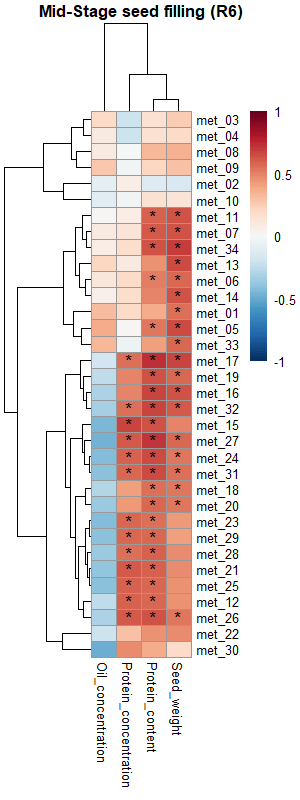
\includegraphics[keepaspectratio]{outputs/figures/heatmap_R6.png}}
\end{center}




\end{document}
